\documentclass[a4paper, 11pt]{article}
\usepackage{comment} % enables the use of multi-line comments (\ifx \fi) 
\usepackage{lipsum} %This package just generates Lorem Ipsum filler text. 
\usepackage{fullpage} % changes the margin
\usepackage{hyperref}
\usepackage{graphicx}

\begin{document}
%Header-Make sure you update this information!!!!
\noindent
\large\textbf{Assignment 6} \hfill \textbf{Tyler Wilding} \\
\normalsize COSC 4426 \hfill Due Date: 30/10/16 \\
Prof. Biocchi \hfill -- \\
TA: -- \hfill --

\section*{Descriptions of Systems}
The four systems that I chose to discuss are:
\begin{itemize}
\item Home PC
\item ThinkPad Laptop
\item DigitalOcean Server
\item Phone
\end{itemize}

\subsection*{Operating System}
In terms of their opreating systems, these systems are quite different.  The ThinkPad Laptop is running the latest version of Linux Mint 18, a distribution of Linux very similar to ubuntu and also the most popular linux distribution. The DigitalOcean server is running Ubuntu 16.04, the long-term support and latest version of ubuntu.  Like Linux Mint, ubuntu is a very popular distribution of linux and server oriented versions of Linux always have curated packages to ensure stability and prioritize the efficiency and performance of the server wherever possible.  My home PC is using Windows 10 updated to the latest version, and the mobile phone is using Android 6.0.1 with a custom ROM called Chroma.

\subsection*{Code Base}
Both the ThinkPad and the DigitalOcean server are running Linux, therefore their main codebase is going to be in C as this is what the Linux Kernel is programmed in and many of the popular packages and additions that run ontop of the kernel.  While Android phones do use the Linux Kernel as well, it is more relevant to consider it's code base Java, as it is Java that is used in all of the apps and functionality for the device and would most likely be the code to attempt to break if you were a hacker.  Lastly, the Windows 10 home computer's code base will be C / C++ and some C\#, as these are the main languages used by Microsoft; however C\# may not be used as much as the former.  It is worth mentioning that both Linux and Android are open source, while Windows is not.

\subsection*{Vulnerabilties}
For many of these systems, the vulnerabilities are too lengthy to list as well as many are undiscovered.  In terms of the linux systems, the main vulnerabilities often arise on the main packages that run ontop of the system.  If these packages are compromised and are an integral part of the overall system then it can be very easy for a hacker to make access.  For example, a misconfigured MySQL database can allow a hacker to gain access to the file system.  One of the largest vulnerabilities that happens on an android phone would probably be malicious apps.  This is even worse when on a rooted phone like mine as it allows for the user as well as programs to modify files that can be device-breaking if done incorrectly.  Lastly, the Windows 10 computer is alright, however some of the biggest vulnerabilties are not from the large collection of potential viruses, but rather how all of the new cloud features that invade your privacy are running in the background, creating another way for a malicious user to get access.

\subsection*{Security Features}
The Android phone is the only system that does not require a password before using the system.  Android phones have many security features, the phone can be encrypted, tracked via GPS, and the lock-screen can be protected as well.  However, it is only a phone and as a result the security options are rather slim and limited in comparison to a more traditional device.   For the home computer with Windows 10, the built-in anti-virus is much better than previous versions of Windows, to the point where an external anti-virus is not really required.  Windows 10 also adds a lot of security features including Device Guard which is intended to prevent Zero-Day attacks, Secure Boot prevents attacks from running unsigned images on the computer at boot time.  And last but not least, the default browser Edge is a huge improvement is security as compared to Internet Explorer.  Ubuntu and Mint (which is just essentially a derivative of ubuntu) has many security features and packages that enhance the security.  The main portions of a linux system that need protecting is the remote accessing, user accounts, and filesystem encryption.  Linux has a built in firewall and can be used to modify the port permissions.  Additionally user accounts in linux have their passwords hashed, and as a multi-user environment allows permissions for what users can access or modify.  More detail about what features ubuntu offers is available \href{https://wiki.ubuntu.com/Security/Features}{Here}

\subsection*{Access Method or Location}
Both the laptop and the Android phone are often on my person and are accessed by physically using the device.  The home PC is also accessed physically.  However the DigitalOcean server can only be accessed remotely and is located in a secure datacenter in Toronto.

\subsection*{Usecase}
The laptop is mostly used for school work and as a result contains fairly unimportant information to someone else.  However the phone and home pc would contain more personal information and may be of interest to malicious attacks.  The DigitalOcean server is used for running websites which at the moment are being shared by four people that all have sudo access.

\section*{Risk Probability}
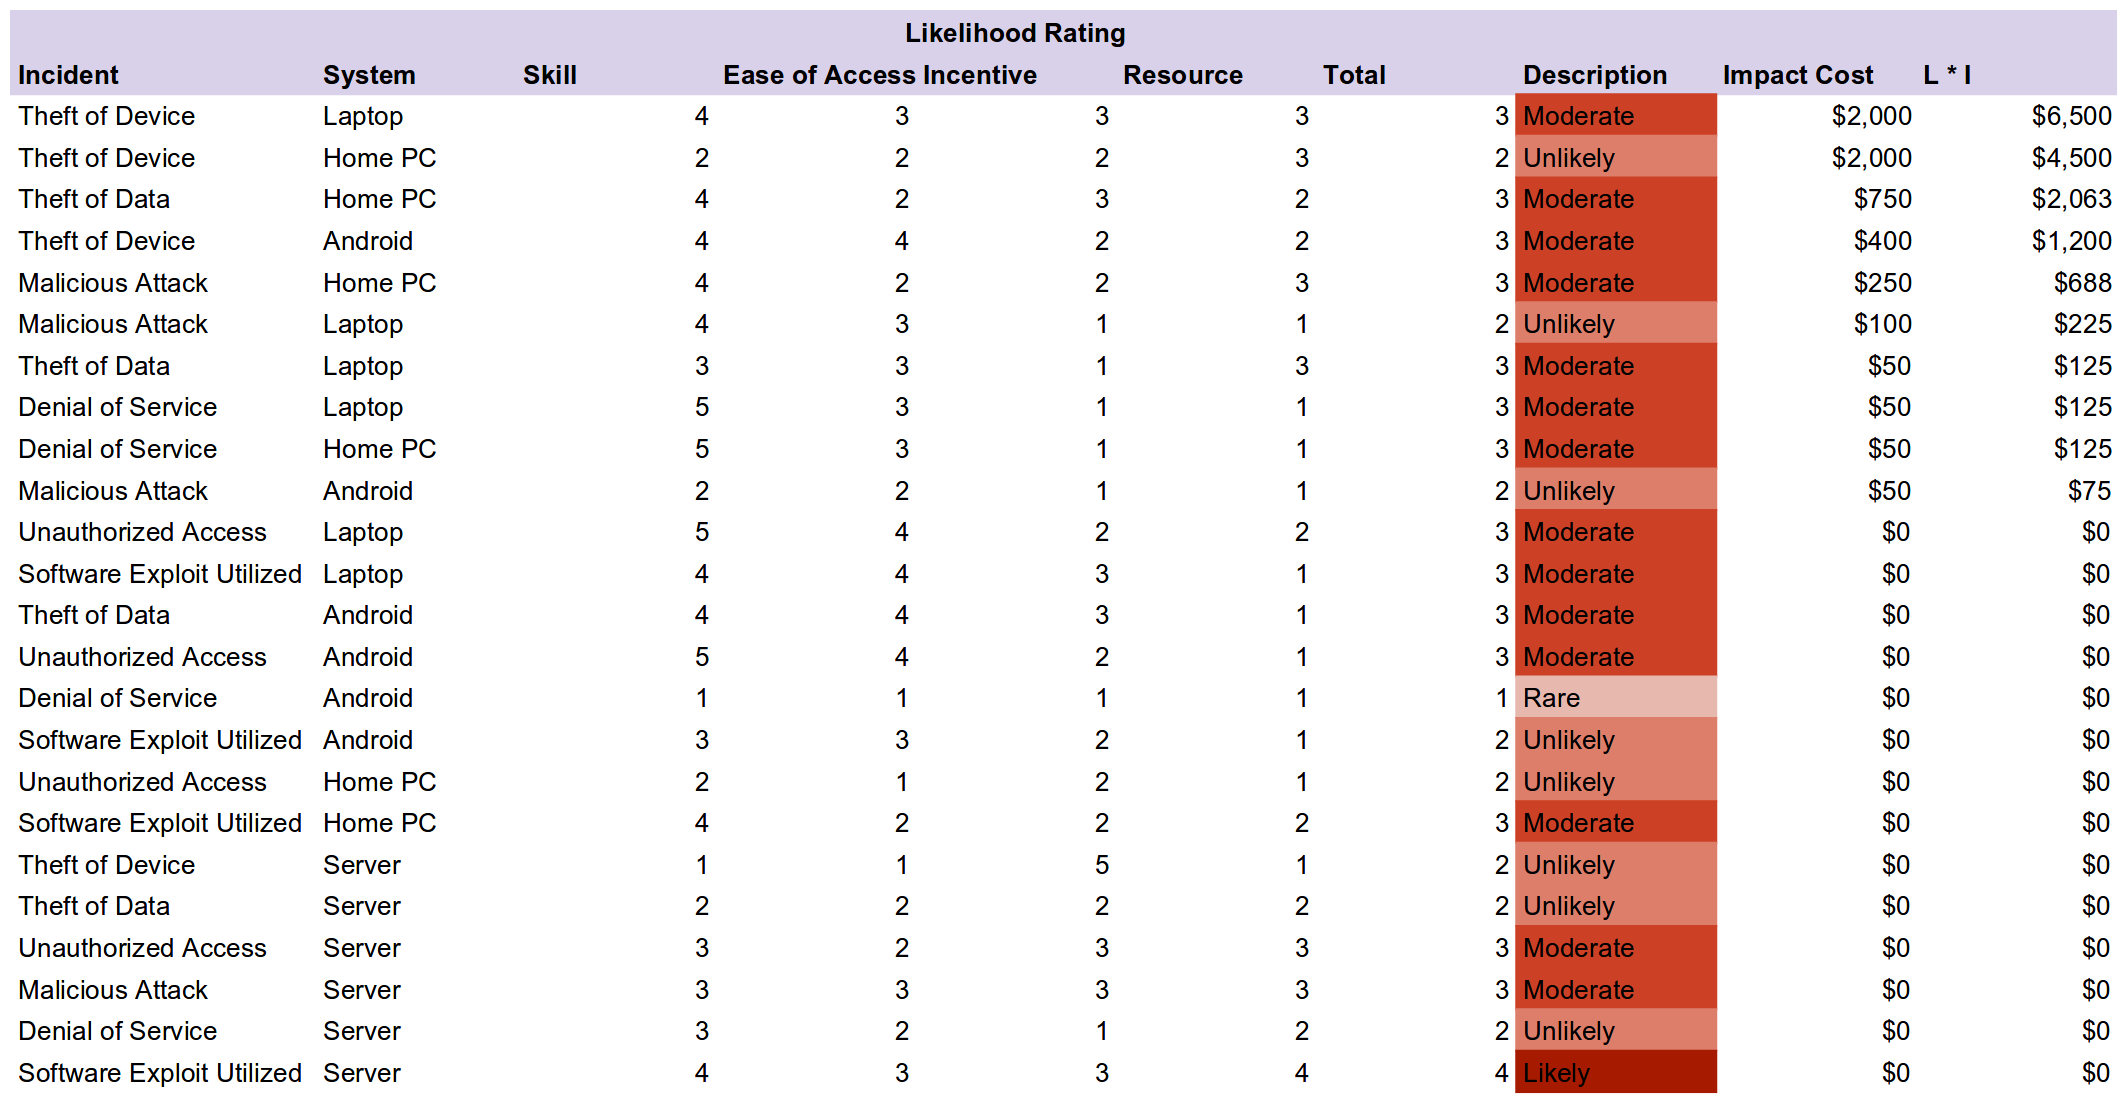
\includegraphics[scale=0.21]{risk.png}

Determination of risk is a difficult thing to do, especially since the majority of these incidents would just be an inconvienance.  The most expensive risks for me are having my devices stolen, as the replacement cost and the fact that I care my phone and laptop a lot in public, lead this to be a fairly high risk.  However in comparison, most other attacks do not inconvience myself very much.  For example if only data was stolen from my laptop I could get it up and running again in only a few hours.  One interesting thing is how the DigitalOcean server has very little costs, this is because all of the costs are absorbed by DigitalOcean.  If something goes wrong, I simply make a new server instance.  DigitalOcean is particularly risky for me because the account is currently being shared by several people as well as the IP range is fairly popular and will easily be hacked if you misconfigure something.  The other issue with the server is that I do not get the security updates as often as I should.\\

It is fairly trivial for an attacker to launch a malicious atack onto a windows computer, as compared to a mobile computer in my opinion.  This is because Windows has a history of being the more easier target to attack, and therefore it has the largest amount of people that try to exploit these flaws in Windows.  It is quite difficult to do the same kind of attacks onto a mobile phone as it is a conventional computer, for example a denial of service attack onto a specific phone would be diffcult as you are always moving around and changing IPs.\\

\section*{Risk Factors}
Part of the reason why some of the devices are prone to a lot of risk are the following.  The Android phone does not use a lock screen and is carried in public as as such it is susceptible to being affected by many people.  Likewise, while my laptop does have a password, it is also on my person in public a lot and physical access is root access, even if it is running Linux.  Thirdly, the DigitalOcean server is being shared by 4 or 5 people right now and anything would be done incorrectly by one of them and cause the computer to be compromised.  Lastly, the home PC, while locked up inside my house and having a password, could be compromised from anything from someone entering my house, to a virus online, to a security vulnerability.

\section*{Risk Conclusion}
In the end calculating risk is a very subjective thing, and many of my estimates were difficult to make because you don't know what will happen, how easy it is, or even how bad it will be to recover from until the incident actually occurs.  This is one of the problems with developing a security plan to pitch to higher-ups that we discussed in class, and it is quite obvious here.

%
%\begin{thebibliography}{9}
%\bibitem{Robotics} Fred G. Martin \emph{Robotics Explorations: A Hands-On Introduction to Engineering}. New Jersey: Prentice Hall.
%\bibitem{Flueck}  Flueck, Alexander J. 2005. \emph{ECE 100}[online]. Chicago: Illinois Institute of Technology, Electrical and Computer Engineering Department, 2005 [cited 30
%August 2005]. Available from World Wide Web: (http://www.ece.iit.edu/~flueck/ece100).
%\end{thebibliography}

\end{document}
